\documentclass[a4paper,12pt]{article}
\usepackage{srcltx}
\usepackage[colorlinks=false,pdfborder=000]{hyperref}
\usepackage{enumerate}
\usepackage{multirow}
\usepackage{titling}
\usepackage[top=1.1in, bottom=1.1in, left=1.2in, right=1.2in]{geometry}
\usepackage[dvips,pdftex]{graphicx,color}
\DeclareGraphicsRule{*}{eps}{*}{}
\usepackage{times}
\usepackage{comment}
\usepackage{subfigure}
\usepackage{amssymb}
%\usepackage[ruled]{algorithm2e}
\usepackage{algorithm}
\usepackage{algorithmic}
\usepackage{subfigure}

%%%%%%%%%%%%%%%%%%%%%%%%%%%%%%%%%%%%%%%%%%%%%%%%%%%%%%%%%%%%%%%%%%%%%%%%%%%%%%%%
\newcommand{\CSE}{\href{http://www.cse.cuhk.edu.hk}{Department of Computer Science and
Engineering}}
\newcommand{\CUHK}{\href{http://www.cuhk.edu.hk}{The Chinese University of Hong Kong}}
\newcommand{\mymail}{\mbox{\textcolor{blue}{\underline{zgxiao@cse.cuhk.edu.hk}}}}
\newcommand{\myname}{\href{http://www.cse.cuhk.edu.hk/~zgxiao}{XIAO Zigang}}
\newcommand{\header}[1]{\noindent {\bf \\#1\\}}
\renewcommand{\algorithmiccomment}[1]{//#1}
%%%%%%%%%%%%%%%%%%%%%%%%%%%%%%%%%%%%%%%%%%%%%%%%%%%%%%%%%%%%%%%%%%%%%%%%%%%%%%%%
\pretitle{\begin{center}\bf \LARGE} \posttitle{\par\end{center}}
\preauthor{\begin{center}
            \small \lineskip 0.5em%
            \begin{tabular}[t]{c}}
\postauthor{\end{tabular}\par\end{center}}
\predate{\begin{center}\small} \postdate{\par\end{center}}
%%%%%%%%%%%%%%%%%%%%%%%%%%%%%%%%%%%%%%%%%%%%%%%%%%%%%%%%%%%%%%%%%%%%%%%%%%%%%%%%
\title{CEG5270 Assignment 1 (2009 Spring)}
\author{\myname\\\mymail\\\CSE\\\CUHK}
\date{\today}

%%%%%%%%%%%%%%%%%%%%%%%%%%%%%%%%%%%%%%%%%%%%%%%%%%%%%%%%%%%%%%%%%%%%%%%%%%%%%%%%
\begin{document}
\maketitle
\begin{enumerate}
\item
Use greedy algorithm to solve this problem.\\
\begin{algorithm}[htbp!]
\caption{Find chromatic number of interval graphs}
\begin{algorithmic}[1]
\STATE Sort the start and end point of intervals, save it in a list $L$.
\STATE Mark all intervals as not colored.
\STATE freelist $\leftarrow \{1,2,...,n\}$, usedlist $\leftarrow \varnothing$, $k \leftarrow 0$
\FOR {$i=1$ to $2n$}
    \IF {$L_i$ is start point of interval $x$}
        \STATE $c \leftarrow $ head of freelist
        \STATE $x$.color $\leftarrow$ $c$
        \STATE freelist $\leftarrow$ freelist $- \{c\}$
        \STATE usedlist $\leftarrow$ $\{c\} \cup$ usedlist
        \IF {$c > k$}
            \STATE $k \leftarrow c$
        \ENDIF
    \ELSE [ $L_i$ is end point of interval $x$ ]
        \STATE $c \leftarrow $ $x$.color
        \STATE usedlist $\leftarrow$ usedlist $- \{c\}$
        \STATE freelist $\leftarrow$ $\{c\} \cup$ freelist
    \ENDIF
\ENDFOR
\RETURN  $k$.
\end{algorithmic}
\end{algorithm}


Proof: Let $x$ be the vertex which is colored to $k$. Since $x$ is not colored to a smaller value,
it means $x$'s start point $a$ intersects with the intervals which are colored from $1$ to $k-1$,
i.e. those intervals includes $a$. Then these intervals forms a $k-$clique.
Hence $\omega(G) \geq k \geq \chi(G)$.But we know that $\chi(G) \geq \omega(G)$.
Hence $\omega(G) = \chi(G) = k$.

Complexity: Sorting $2n$ elements takes $O(n\log n)$.
And it takes $O(n)$ for the for loop in the algorithm, only $O(1)$ for the inserting and removing operation of queues.
Hence the total complexity is dominated by the sorting time $O(n\log n)$.
%%%%%%%%%%%%%%%%%%%%%%%%%%%%%%%%%%%%%%%%%%%%%%%%%%%%%%%%%%%%%%%%%%%%%%%%%%%%%%%%
\item
Let $H[k][i][j]$,$V[k][i][j]$ denote the number of at most K multi-bend routes
from s to t where the last step is horizontal move and vertical move, respectively. And:
\begin{equation}
H[k][i][j] = \left\{ \begin{array}{ll}
            0   &   \textrm{if $j=0$ or $i\neq0 \wedge j\neq0 \wedge k=0$}\\
            1   &   \textrm{if $j\neq 0 \wedge i=0 $}\\
            H[k][i][j-1] + V[k-1][i][j-1]&  \textrm{otherwise}\\
                    \end{array}\right.
\end{equation}
\begin{equation}
V[k][i][j] = \left\{ \begin{array}{ll}
            0   &   \textrm{if $i=0$ or $i\neq0 \wedge j\neq0 \wedge k=0$}\\
            1   &   \textrm{if $i\neq 0 \wedge j=0 $}\\
            H[k-1][i-1][j] + V[k][i-1][j] & \textrm{otherwise}\\
                    \end{array}\right.
\end{equation}
Without loss of generality, let $(0,0)$ and $(x,y)$ be the coordinate of $s,t$,
then $H[k][x][y]+V[k][x][y]$ is the number of multi-bend routes from s to t.
%%%%%%%%%%%%%%%%%%%%%%%%%%%%%%%%%%%%%%%%%%%%%%%%%%%%%%%%%%%%%%%%%%%%%%%%%%%%%%%%
\item
\begin{enumerate}[(i)]
\item
~\\
\begin{algorithm}[htbp]
\caption{Computer coordinate of PE modules}
\begin{algorithmic}[1]
\STATE Define a tree structure where each subtree represent a block
\STATE Initialize each operand and operator as a tree node
\FOR [construct the tree from the normalized expression $\alpha$] {$i=1$ to $2n-1$}
    \IF {$\alpha_i$ is an operand}
        \STATE stack.push($\alpha_i$)
    \ELSE [$\alpha_i$ is an operator]
        \STATE b $\leftarrow$ stack.pop(), a $\leftarrow$ stack.pop()
        \STATE construct a new node where  $\alpha_i$ is the parent and a,b is the children
    \ENDIF
\ENDFOR
\STATE head $\leftarrow$ stack.pop()
\STATE BFS(head) //use a BFS to compute the corner of each block.
\end{algorithmic}
\end{algorithm}

\begin{algorithm}[htbp]
\caption {Function BFS(head)}
\begin{algorithmic}[1]
\STATE queue.enque(head)
\WHILE{queue not empty}
    \STATE node $\leftarrow$ queue.pop\_head()
    \STATE L $\leftarrow$ node.left\_child, R $\leftarrow$ node.right\_child
    \IF {node == `*'}
        \STATE L.(x,y) $\leftarrow$ (node.x, node.y)
        \STATE R.(x,y) $\leftarrow$ (node.x + L.width, node.y)
        \STATE queue.enque(L), queue.enque(R)
    \ELSIF {node == `+'}
        \STATE L.(x,y) $\leftarrow$ (node.x, node.y)
        \STATE R.(x,y) $\leftarrow$ (node.x, node.y + L.height)
        \STATE queue.enque(L), queue.enque(R)
    \ENDIF
\ENDWHILE
\end{algorithmic}
\end{algorithm}
Analysis:

In the first step, we traverse the polish expression to construct the tree, which takes $O(n)$ time.
After the tree is constructed, the BFS also takes $O(n)$ time because there are $n-1$ operators(internal nodes) in the tree.
Hence the total run time of the algorithm is $O(n)$.
\item
Proof:

The first move ensures that given $n$ operands,
we can switch any two operands by one or more such moves,
i.e. we can get all permutations of operands;

The third move ensures that operator can switch to any `slot' between two operands(may not be valid polish expression).
Also note that we could always generate a polish expression in the form $p_1p_2e_1p_3e_2...p_ne_{n-1}$, i.e.
all operator forms a chain of size $1$ by itself.
Then using the second move, we can generate all possible combination$(=2^{n-1})$ of operators.
By combining the third second move,
we can generate all possible permutation of operators.

Since every valid normalized polish expression is corresponds to a slicing floorplan,
which means the solution space is a subset of the possible string generated by the three moves,
hence the reachability is ensured.
\end{enumerate}
%%%%%%%%%%%%%%%%%%%%%%%%%%%%%%%%%%%%%%%%%%%%%%%%%%%%%%%%%%%%%%%%%%%%%%%%%%%%%%%%
\item
\begin{enumerate}[(i)]
\item
$C:$ $q[j]<i$ and no edge between $q[j]$ and $Largest$\\
$D:$ $Largest=q[j]$

Explanation: Condition $C$ means that if for some number $x=q[j]<i$,
then they have the relationship like $(...x...i...),(...x...i...)$ in the sequence pair.
Also it checks if it will be a transitive edge.
Statement $D$ helps to update the $Largest$ so as to keep track of the transitive edge information.
\item
Change line 3 to:\\
\textit{3: For(j=k+1 up to n) do}

Replace every occurrence of $G_h$ to $G_v$ in the pseudo code.
\item
Since every pair of modules has a binary relation, the total number of edges would be $C^2_n$ with transitive edges.
In the worst case of horizontal constraint graph, all the modules are placed one next to another.
But if transitive edges are removed there will be at most $(n-1)$ edges.
This result holds in vertical constraint graph.
Hence the number of edges in the constraint graph can be reduce to $O(n)$.
\end{enumerate}
%%%%%%%%%%%%%%%%%%%%%%%%%%%%%%%%%%%%%%%%%%%%%%%%%%%%%%%%%%%%%%%%%%%%%%%%%%%%%%%%
\item
\begin{enumerate}[(i)]
\item
    \begin{enumerate}[For 1:]
        \item (4,12), (6,8), (8,6), (12,4)
        \item (10,10)
        \item (4,7), (7,4)
        \item (3,8), (4,6), (6,4), (8,3)
    \end{enumerate}
\item
    See Figure \ref{fig:shape}.
    \begin{figure}[!htbp]
    \centering
    \subfigure[1]{\label{fig:1}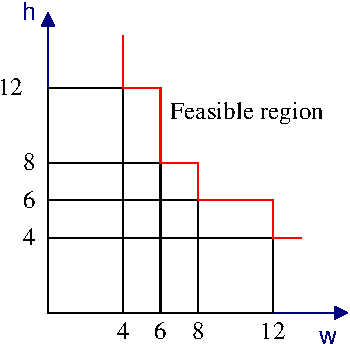
\includegraphics[width=0.24\textwidth]{p5_1.pdf}}
    \subfigure[2]{\label{fig:2}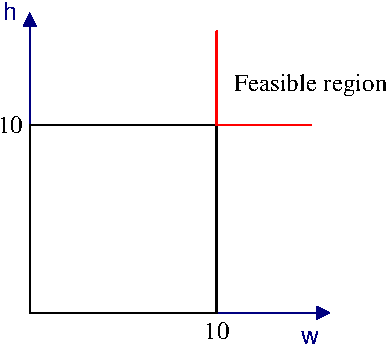
\includegraphics[width=0.24\textwidth]{p5_2.pdf}}
    \subfigure[3]{\label{fig:3}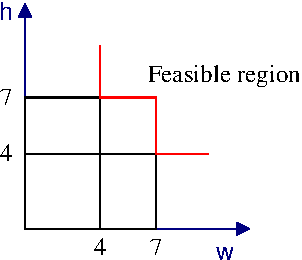
\includegraphics[width=0.24\textwidth]{p5_3.pdf}}
    \subfigure[4]{\label{fig:4}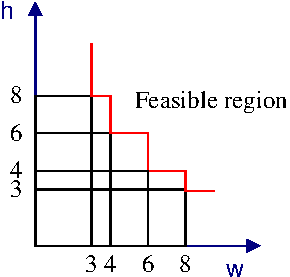
\includegraphics[width=0.24\textwidth]{p5_4.pdf}}
    \subfigure[23*]{\label{fig:23}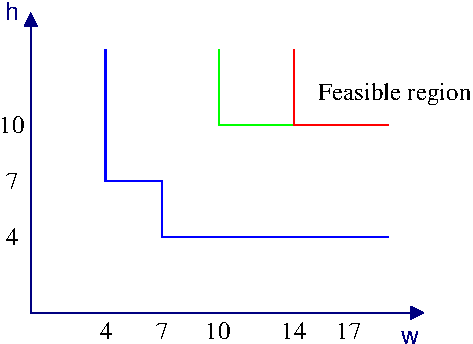
\includegraphics[width=0.3\textwidth]{23x.pdf}}
    \subfigure[123*]{\label{fig:123}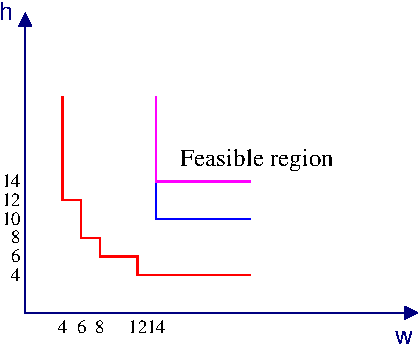
\includegraphics[width=0.3\textwidth]{123x+.pdf}}
    \subfigure[123*+4*]{\label{fig:1234}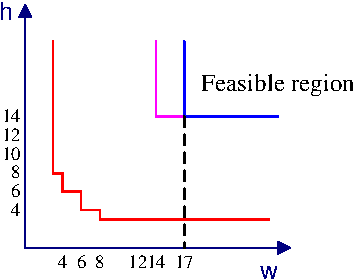
\includegraphics[width=0.3\textwidth]{123x+4x.pdf}}
    \caption{shape curves}
    \label{fig:shape}
    \end{figure}
\item
    According to the shape curve of $123*+4*$, the width and height of the smallest packing should be $17\times14$ .
\end{enumerate}


\end{enumerate}
\end{document}
